\section{Methodology}


In this section, we will show the details of the self-supervised InfNet for imaging segmentation model including the network architecture, the data preprocessing steps, and the loss function. We will show how self-supervised InfNet helps to improve generalization and performance of the model while having a limited number of data samples. We will also show the extension of our data preprocessing steps which further improves the performance of our model.

Supervised InfNet (Lung Infection Segmentation Network) will be used as our baseline to compare without using any semi-supervised learning algorithm. This is to show that the self-supervised learning method improves the performance of the baseline supervised learning InfNet for imaging segmentation. We will extend our work on supervised InfNet by adding self-supervision method to it.

We will not change the structure of the InfNet model and use the default parameters as included in their GitHub code. There will be two different types of the InfNet model - single InfNet and multi InfNet. 

The single InfNet will create a single-labeled segmentation of the image for the infected region. The single InfNet predicts if the region is either ground-glass opacities or consolidations. It represents ground-glass opacities or consolidations as the same label. This means that the single InfNet will only predict the infected region without classifying them more specifically.  The CT lung image is first passed into the initial convolutional layers of the single InfNet to extract the features of the CT lung image. Then, the features generated from the convolutional layer are fed into the partial decoder module, reverse attention module, and the edge detection module. The edge detection module is to help the network with the detection of the boundaries of the segmentation. The reverse attention and the partial decoder generates the segmentation of the infection regions of the CT lung images.

The prediction from the single InfNet represents the infected region and will act as a prior to be fed into the multi InfNet. The prior will be concatenated with the original CT image to be fed into the multi InfNet network. The multi InfNet network will be used to predict multiple-labeled segmentation. The multiple-labeled segmentation includes predicting the background, ground-glass opacities, and consolidations for the infected region. The multiple-labeled segmentation model will give each of the labels a different value instead of grouping them as one as what the single-segmentation model does.

\subsection{Self-supervised InfNet for imaging segmentation}

We will propose using a self-supervised method to improve the performance of deep neural networks to create pixel-level segmentation for CT scans for lung images of COVID-19 patients. We will integrate self-supervised inpainting to pre-train our network. Since image inpainting is similarly related to image segmentation, we will integrate the pre-training steps as image inpainting for our image segmentation network. 

The original InfNet model would generate 5 different predictions: the edge segmentation prediction and the other 4 are segmentation of the infected regions but of different sizes. To utilize the ability of self-supervised method for InfNet segmentation, we generate masks to be fed into the InfNet model. The last convolution layer that outputs the prediction is not used for the self-supervised case. However, the last convolutional layer is replaced with a different convolutional layer to reconstruct the image and the edge appropriately. Everything else is kept the same as the InfNet architecture. This way the network will learn meaningful representations of the CT images and we can use these meaningful representations to learn the segmentation of the infected regions of the CT lung images. After learning the self-supervised features for InfNet, the training continues as normal similar to the InfNet algorithm. The training will start with the weights trained using the self-supervised inpainting method. The last layer will be changed to its original layer instead of the replaced convolutional layer. 

By learning features from image inpainting, the model can learn more features that are related to image segmentation. As creating masks can be a complex task for the network to learn to inpaint, the mask can either be too complex for the network to start learning or too simple to be able to learn good representations. We will be using a coach network that increases the complexity of the masking of the CT images throughout the training of the network. The mask created will initially be relatively simple, once the network can predict the inpainting of the CT images with good performance, the coach will increase the complexity of the masking to reduce the performance of the network, similar to how Generative Adversarial Network (GAN) works. The loss for the coach network is constructed from the loss of the image inpainting from the InfNet. The coach network and the InfNet both work together as a MinMax algorithm. The InfNet will try and minimize the loss to generate better image inpainting while the coach network will try to increase the loss of the image inpainting through generating more complex masks. In the beginning, the masks generated by the coach network will be less complex. Through the training of the coach network, as the InfNet gets better at predicting image inpainting, the coach network will generate more complex masks. The loss fuction for the coach network is:
\begin{equation}
L_{coach}(x) = 1 - L_{rec}(x\odot M)
\end{equation}

where $M = C(x)$ which is created by the coach network. A constraint is applied to this loss function because the coach network would just create a mask that masks all regions. After all, noa context information would be present for the network to learn and a maximum loss will be achieved. The constraint is:
\begin{equation}
\hat{B}(x) = B(x) - SORT(B(x))^{k|B(x)} 
\end{equation}
\begin{equation}
M = C(x) = \sigma (\alpha \hat{B}(x))
\end{equation}

The backbone, B, of the coach network has a similar network architecture with the model that inpaints the CT images. SORT(B(x)) sorts the features in descending order over the activation map. k represents the $k^{th}$ elements in the sorted list and k helps to control the fraction of the image to be erased. The region that has scores lesser than the $k^{th}$ element will be erased from the images. If k is 0.75 then 0.75 fraction of the images will not be erased. The score is scaled into a range of [0, 1] using a sigmoid activation function. We keep $\alpha = 1$ while training the coach network.
The illustration of the coach network can be seen in \ref{fig:coach-arch}.

\begin{figure*}
	\centering
	\small
	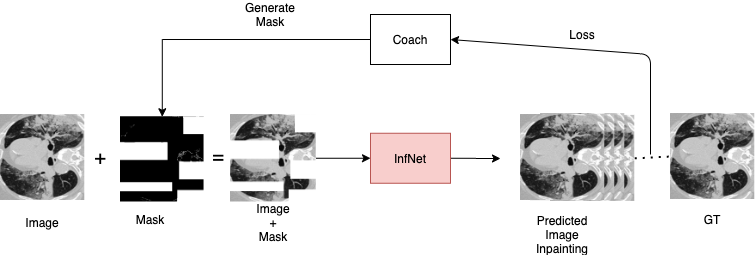
\includegraphics[width=\linewidth]{coach.png}
	\caption{The architecture of the coach network for self-supervised inpainting. }
	\label{fig:coach-arch}
\end{figure*}

After the self-supervision training is finished, the single segmentation InfNet would reuse the self-supervised single InfNet network weights to train normally on the segmentation of the CT lung images. Likewise, the multi InfNet network would reuse the weights that were trained during self-supervised multi InfNet training to train normally on the segmentation of the CT lung images.

The proposed self-supervised single-labeled segmentation InfNet network architecture can be seen in \ref{fig:inf-net_arch}. The left side of the figure is the original Single InfNet architecture and the right side of the figure is the self-supervised Single InfNet. The last layer for each output prediction is replaced with a different linear activation layer. The linear activation layer will re-create the original image that is covered by the masks. 

\begin{figure*}
	\centering
	\small
	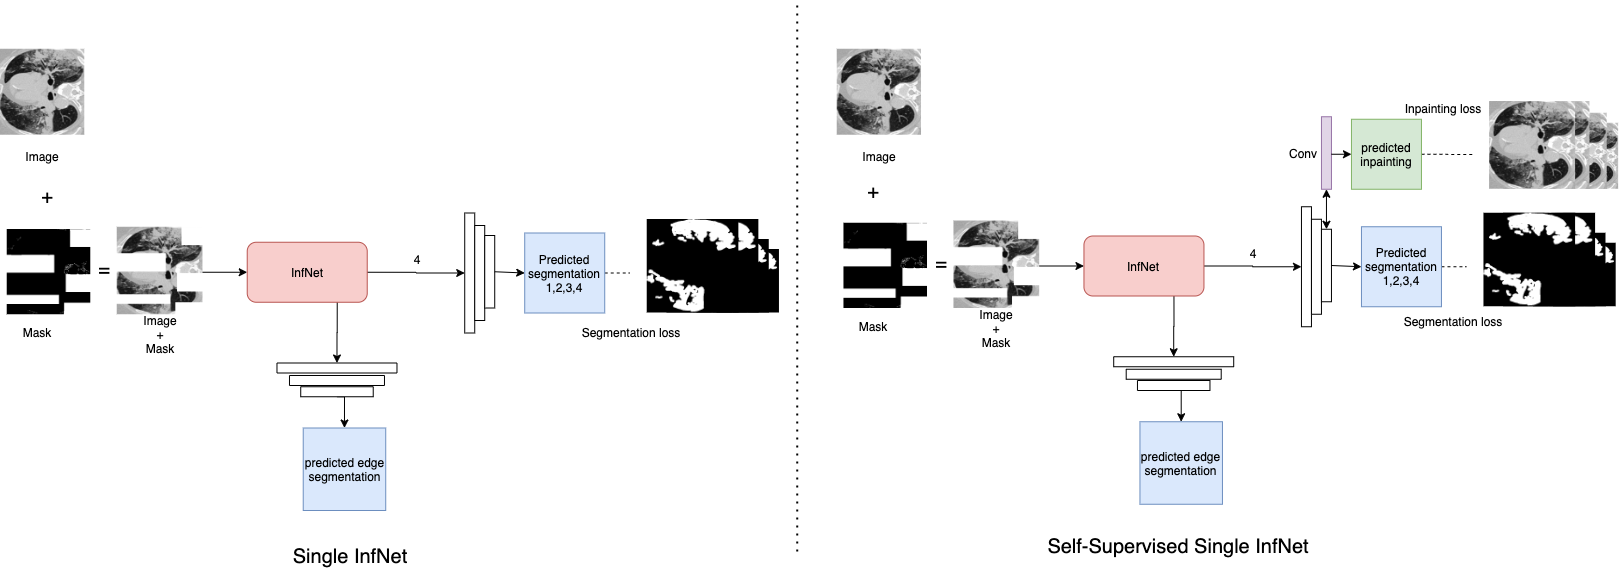
\includegraphics[width=\linewidth]{self-super-inf-net.png}
	\caption{The architecture of our self-supervised InfNet model. }
	\label{fig:inf-net_arch}
\end{figure*}


The proposed self-supervised multi-labeled segmentation InfNet network architecture is shown in \ref{fig:multi-inf-net_arch}. The changes in the architecture for the multi-labeled segmentation InfNet are similar to the single-labeled segmentation InfNet where the last layer of the layer is replaced with a different linear activation layer to output the inpainting of the original image. 

\begin{figure*}
	\centering
	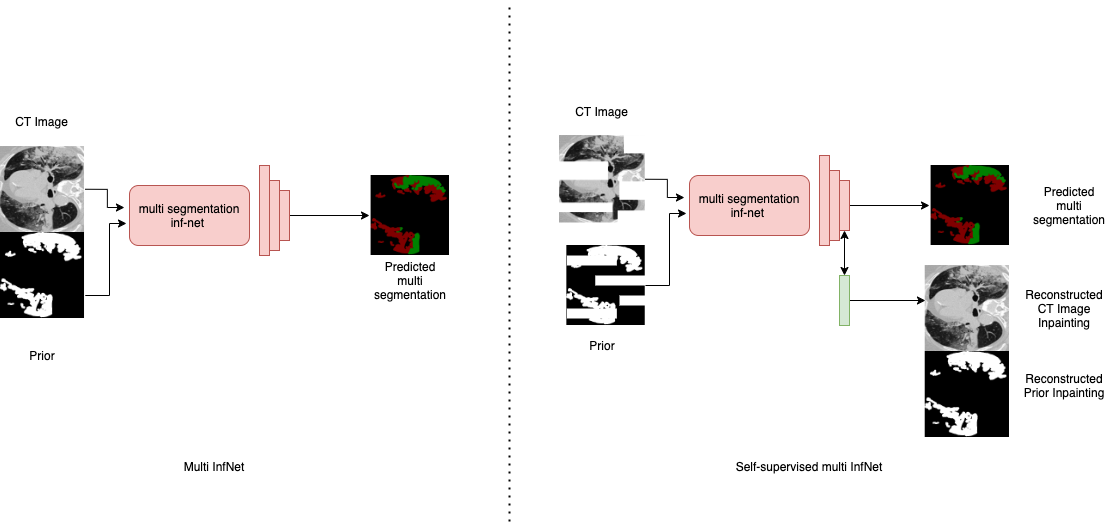
\includegraphics[width=\linewidth]{self-super-multi-inf-net.png}
	\caption{The architecture of our self-supervised multi segmentation InfNet model. Highlighted green block is the difference between the original multi InfNet and our self-supervised multi InfNet.}
	\label{fig:multi-inf-net_arch}
\end{figure*}

\begin{algorithm}
	\caption{Pseudo code for self-supervised with InfNet}
	\label{alg:self-inf-net}
	\begin{algorithmic}
		\STATE \textbf{Input:} $D_{labeled}$ = [($inputImage_1$, $G_{t1}$), ...]
		\FOR {each epoch}
		\FOR{each coach step}
		\STATE mask = M(x)
		\STATE maskedInput = $mask \odot inputImage$
		\STATE $ predictedImage =network(maskedInput), inputImage$
		\STATE $L_{rec} = CrossEntropy(predictedImage, inputImage)$
		\STATE $L_{coach}(x) = 1 - L_{rec}$
		\STATE update coach weights
		\ENDFOR
		\FOR {each network step}
		\STATE $P_{labeled} = Preprocess(D_{labeled})$
		\STATE $inpaintingOutput = network(P_{labeled})$
		\STATE $L_{rec} = CrossEntropy(InpaintingOutput, inputImage)$
		\STATE backpropogate and save network weights
		\ENDFOR
		\ENDFOR 
		
		
		\FOR {each batch of $D_{labeled}$:}
		\STATE $P_{labeled}$ = Preprocess ($D_{labeled}$)
		\STATE $trainLoss = train(P_{labeled})$
		\STATE Backpropagate train loss
		\STATE $testLoss = test(P_{labeled})$
		\STATE save model weights, \textit{w}.
		\ENDFOR
	\end{algorithmic}
\end{algorithm}

The output of the single segmentation InfNet will include the edge of the segmentation and four single-labeled segmentation of the infected region of the CT lung images with different sizes as shown in \ref{fig:supervised-inf-net_arch}. A loss will be calculated for each of the outputs from the single InfNet model. The first loss function is the loss edge, $L_{edge}$ which guides the model in representing better segmentation boundaries. The other loss function is the segmentation loss, ${L_{seg}}$. The segmentation loss combines both the loss of Intersection over Union (IoU) and the binary cross entropy loss. The segmentation loss equation for the single InfNet is as follow:
\begin{equation}
L_{seg} = L_{IoU} + \lambda L_{BCE}
\end{equation}

\begin{figure}
	\small
	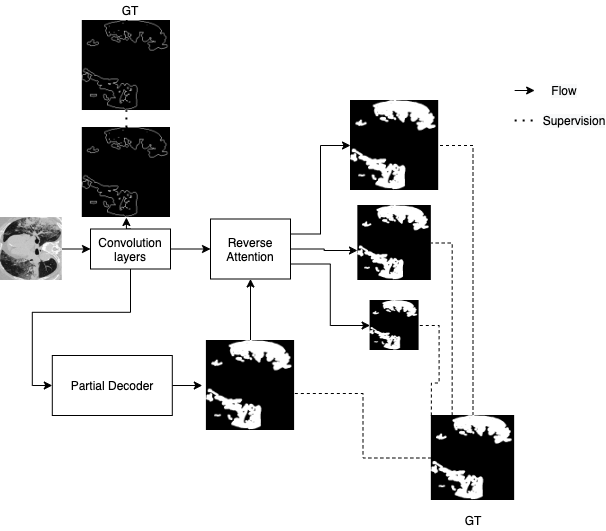
\includegraphics[width=88mm]{supervised-inf-net.png}
	\caption{Architecture of the supervised InfNet.  }
	\label{fig:supervised-inf-net_arch}
\end{figure}

The $\lambda$ is set to 1 for this experiment. The segmentation loss is adapted to all of the ${S_i}$ predicted output where ${S_i}$ are created from $f_i$ such that $i={3,4,5}$. 

The total loss function for the single InfNet model is then:
\begin{equation}
L_{total} = L_{seg}(G_t, S_g) + L_{edge} + 	\sum_{i=3}^{5}L_{seg}(G_t, S_i)
\end{equation}

The summation of the loss functions are calculated from the output of the three convolutional layers. $G_t$ refers to the ground truth labels. $S_g$ is the output from the parallel partial decoder to match with the ground truth label.

As for the multiple segmentation infected region InfNet. We also use the default model and hyperparameters from the InfNet code. We will however train the network without using any unlabeled images to be used as a supervised version. The CT lung images and prior (infected region) for the CT lung images are concatenated together before being fed into the multiple segmentation InfNet. The prior is generated from the single segmentation InfNet. The prior would contain the area of the infected region. However, the prior does not contain the labels for ground-glass opacities and consolidations. It just shows the infected regions. The multiple segmentation InfNet will label the CT lung images with background, ground-glass opacities, and consolidations. The architecture for multiple segmentation InfNet can be seen in \ref{fig:multi-inf-net_arch}. The loss function for the multiple segmentation InfNet is as follow:
\begin{equation}
L_{bce} = \frac{1}{N}\sum_{i=1}^{N} y_i \cdot log(\hat{y_i}) + (1-y_i)\cdot log(1-\hat{y_i})
\end{equation}

The loss function for multiple segmentation InfNet uses the binary cross-entropy between the predicted segmentation and the ground truth segmentation.

In order to improve the performance of the model and to aid in the generalization, we determine to use self-supervised learning to learn good representations of the CT scan of lung images. Self-supervised learning generates auxiliary tasks from the labeled data samples. For instance, when undergoing data augmentation with rotation, we could train the network to predict if the images have been rotated 0 degrees, 90 degrees, 180 degrees to learn representations of the images. 


%determine the severity score of the lung regions through several methods. The severity score of the lungs can be determined by using CT severity score (CT-SS) \cite{ref11}. The score uses lung opacification for extension of the infections in the lungs. CT-SS is an adaptation from the method previously used in patients after severe-acute respiratory syndrome (SARS) \cite{ref10} to describe ground-glass opacity, interstitial opacity, and air trapping. The lungs will be divided into 20 regions, the posterior apical segment of upper left lobe was divided into apical and posterior segmental regions, the anteromedial basal segment of lower left lobe will be divided into anterior and basal segmental regions. For each region, there contain a system attributing scores of 0, 1, 2, either parenchymal opacification involves 0%, less than 50%, or equal to or more than 50%. The CT-SS will calculate the sum of individual scored regions. The final value of CT-SS can range from 0 to 40.


We will compare our method against the supervised %and semi-supervised \cite{ref13,ref14} 
\cite {ref13}models trained on COVID-19 dataset. For comparing supervised learning, we will compare against the paper \cite{ref13}. We will train and follow using the same network structure but change from supervised learning to self-supervised learning and compare the performance between supervised and self-supervised.

%When comparing with the semi-supervised model, we determine that our model is successful if our model is able to reach close to or better than the performance of the semi-supervised model as semi-supervised model is able to obtain a higher amount of data samples by looking at both unannotated and annotated data samples while self-supervised model only have access to the annotated labels. A self-supervised learning method will create its own training annotated labels without any manual human labelling and trained without any unlabeled data samples. We will compare our method’s performance against InfNet \cite{ref14} which uses semi-supervised learning by generating pseudo labels from randomly selected unlabeled CT images.

We will use this approach to determine if self-supervised learning can be a useful task to help InfNet improve its performance in segmenting the ground-glass opacities or consolidation around the infected region of the CT lung images.

%Our method will be novel compare to the other methods mentioned as our method will be integrating both the segmentation of the CT lung images as well as the calculation of the severity score through caluclation of the segmented infected lung areas.



\iffalse
The pseudo-code for the training of baseline model is relatively straightforward as can be seen in \ref{alg:baseline}.
\begin{algorithm}
	\caption{Pseudo code for InfNet}
	\label{alg:baseline}
	\begin{algorithmic}
		\STATE \textbf{Input:} Train data $D_{labeled}$,  test data $D_{t-labeled}$ ground truth $G_t$,
		\FOR {each batch of $D_{labeled}$:}
		\STATE $P_{labeled}$ = Preprocess $D_{labeled}$
		\STATE $L_{seg}(G_t, S_g), L_{edge}, L_{seg}(G_t, S_3), L_{seg}(G_t, S_4), L_{seg}(G_t, S_5)	$  = train(\textit{M},  $P_{labeled}$)
		\STATE $L_{traintotal} = L_{seg}(G_t, S_g) + L_{edge} + L_{seg}(G_t, S_3) + L_{seg}(G_t, S_4) + L_{seg}(G_t, S_5)$
		\STATE plot($L_{traintotal}$)
		\STATE = test(\textit{M}, $D_{t-labeled}$)
		\STATE plot(test loss)
		\STATE save model weights, \textit{w}.
		\ENDFOR
	\end{algorithmic}
\end{algorithm}
\fi 